\documentclass[12pt,letterpaper]{hmcpset}
\usepackage[margin=1in]{geometry}
\usepackage{graphicx}
\usepackage[makeroom]{cancel}
\usepackage{array}
\usepackage{mathtools}
\usepackage{marginnote}
\usepackage{units}
\usepackage{xfrac}
\usepackage{enumerate}
\usepackage{amsmath}
\usepackage{fancyhdr}
\usepackage{pgfplots}
\usepackage{hyperref}
\usepackage{nopageno}
\usepackage{boondox-cal}
\hypersetup{
	colorlinks=true,
	linkcolor=blue,
	filecolor=magenta,      
	urlcolor=magenta,
}

% info for header block in upper right hand corner
\name{} %put your name here
\class{Physics 51 Section \hspace{3mm}} %put your section here
\assignment{Homework 11}
\duedate{Monday, November 9, 2020}

\begin{document}
	\begin{problem}[41E24:]
		In costume jewelry, rhinestones (made of glass with $n = 1.5$) are often coated with silicon monoxide ($n = 2.0$) to make them more reflective.
		How thick should the coating be to achieve strong reflection for 560-nm light, incident normally?
	\end{problem}
	\clearpage



	\begin{problem}[41E30:]
		An oil drop ($n = 1.20$) floats on a water ($n = 1.33$) surface and is observed from above by reflected light (see Fig. 41-26).
		\begin{enumerate}[(a)]
			\item Will the outer (thinnest) regions of the drop correspond to a bright or dark region?
			\item How thick is the oil film where one observes the third blue region from the outside of the drop?
			\item Why do the colors gradually disappear as the oil thickness becomes larger?
		\end{enumerate}
		
		\centering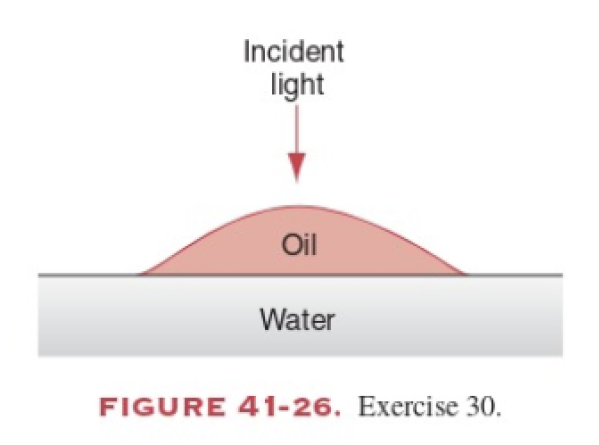
\includegraphics[scale = 0.4]{Fig_41-26}
	\end{problem}
	\clearpage



	\begin{problem}[41E40:]
		An airtight chamber 5.0 cm long with glass windows is placed in one arm of a Michelson interferometer as indicated in Fig. 41-28.
		Light of wavelength $\lambda = 500$ nm is used.
		The air is slowly evacuated from the chamber using a vacuum pump.
		While the air is being removed, 60 fringes are observed to pass through the view.
		From these data, find the index of refraction of air at atmospheric pressure.

		\centering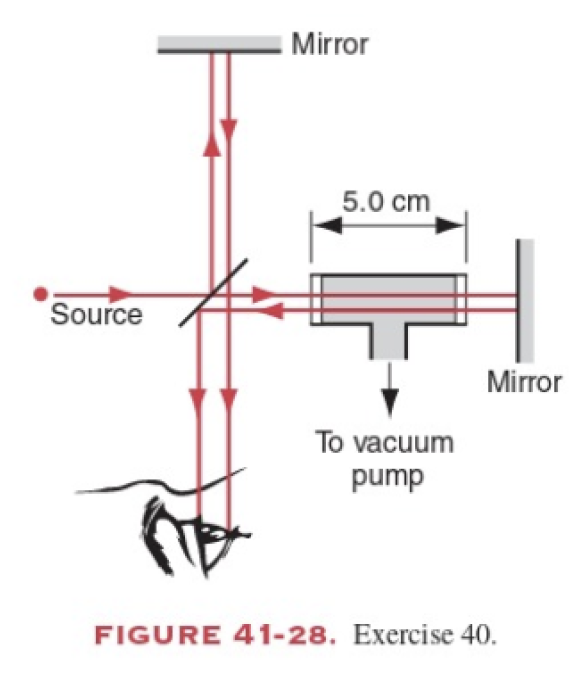
\includegraphics[scale = 0.4]{Fig_41-28}
	\end{problem}
	\clearpage



	\begin{problem}[44E4:]
		Unpolarized light falls on two polarizing sheets placed one on top of the other.
		What must be the angle between the characteristic directions of the sheets if the intensity of the transmitted light is one-third the intensity of the incident beam?
		Assume that each polarizing sheet is ideal—that is, that it reduces the intensity of unpolarized light by exactly 50\%.
	\end{problem}
	\clearpage



	\begin{problem}[44P5:]
		A polarizing sheet and quarter-wave plate are glued together in such a way that, if the combination is placed with face $a$ against a shiny coin, the face of the coin can be seen when illuminated by light of appropriate wavelength.
		When the combination is placed with face $A$ away from the coin, the coin cannot be seen. (a) Which component is on face $A$ and (b) what is the relative orientation of the components?
	\end{problem}
	\clearpage



	\begin{problem}[SUP 11.1:]
		A monochromatic beam of unpolarized light with intensity $I_o$ is incident upon a series of optical elements—polarizers, half-wave plates, and quarter-wave plates.
		In the figure below, the orientations of the transmission axes of the polarizers and the optic axes of the $\lambda/2$ and $\lambda/4$ plates are given with respect to the first polarizer, $P_1$.

		\centering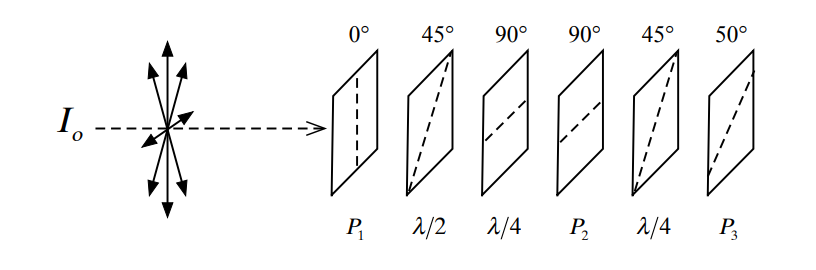
\includegraphics[scale = 0.6]{Sup_11-1}

		\begin{enumerate}[(a)]
			\item What is the intensity after polarizer $P_1$?
			\item After $P_2$?
			\item After $P_3$?
		\end{enumerate}
	\end{problem}
	\clearpage
\end{document}
